\pdfoutput=1

\section{Method}
\label{sec:method}
% \yx{TODO: change according to later content.}
In this section, we present \textbf{Re}inforced \textbf{M}eta-thinking \textbf{A}gents (\method), a RL method integrating meta-thinking into the reasoning process of LLM under multi-agent settings (Sec.~\ref{sec:method.reinforce_ma.deploy_ma}), then describe the learning process enabled by MARL 
% (Sec~\ref{sec:method.reinforce_ma.single_turn}) and propose our GRPO variant for multi-turn LLM interaction (Sec~\ref{sec:method.reinforce_ma.multi_turn}). 
of single- and multi-turn LLM setting (Secs. \ref{sec:method.reinforce_ma.single_turn} and \ref{sec:method.reinforce_ma.multi_turn}).
% and finally we describe how to scale up \method~training (Sec~\ref{sec:method.reinforce_ma.extend_ma}). 
% Discussions about inference-time scaling and reward design are deferred to Appendix~\ref{sec:appx.reinforce_ma.infer_scaling} and \ref{app:reward_design}.
% \wxy{@ziyu: modify the order of appdendix; add intro about the discussions(for what?)}

\subsection{Deploying Meta-Thinking Reasoning Process for LLMs}
\label{sec:method.reinforce_ma.deploy_ma}

Beyond VRP (Sec.~\ref{sec:preliminaries.vrp}), recent studies \citep{muennighoff2025s1,ye2025limo} have shown that integrating meta-thinking behaviors in reasoning process can largely improve the accuracy of the final answers. 
% Meta-thinking is broadly defined as the ability to monitor, control, and evaluate one's cognitive processes \citep{flavell1979metacognition}. 
By integrating Meta-thinking, \method~decomposes problem solving into two sequential phases: a \textbf{meta‑thinking} phase that plans, monitors, or revises strategy, followed by a \textbf{reasoning} phase that produces the detailed solution. 
We analyse Meta-thinking Reasoning Process along two orthogonal axes—\emph{single- vs.\ multi‑agent} and \emph{single- vs.\ multi‑turn}.
% Effective meta-thinking fosters self-awareness, flexible thinking, and adaptive problem-solving, enabling individuals to recognize errors, seek alternative solutions, and optimize performance.

In a single-agent setting, such a process calls LLM once and generates meta-thinking and the following reasoning autoregressively. We formulate the \textbf{meta-thinking reasoning process} (MRP) below:
\begin{equation}
    \mathbf{y} \sim \pi_\theta(\mathbf{y\mid x, m}) \cdot \pi_\theta(\mathbf{m\mid x}),
    \label{eq:mcp1}
\end{equation} 
% \begin{equation} \label{eq:mcp1}
%     \mathbf{y}_T \sim \prod_{t=1}^T \pi_\theta(\mathbf{y}_t\mid \mathbf{x}, \dots,\mathbf{m}_t) \cdot \pi_\theta(\mathbf{m}_t \mid \mathbf{x}, \dots, \mathbf{y}_{t-1})
% \end{equation}
% =(m_1,m_2,\ldots, m_H) =(y_1,y_2,\ldots, y_{H'})
where $\mathbf{m}$ and $\mathbf{y}$ are the output of meta-thinking and reasoning respectively. We present the procedure as shown below:
\begin{equation}
    \mathbf{x} \xrightarrow{\text{meta-thinking}} \mathbf{m}
    \xrightarrow{\text{reasoning steps}} \mathbf{y} 
    \sim
    \mathbf{a}.
    \label{eq:mcp2}
\end{equation}
% \begin{equation}
%     \mathbf{x} \xrightarrow[\pi_h]{\text{meta-thinking}} \mathbf{m}_1
%     \xrightarrow[\pi_\theta]{\text{reasoning}} \mathbf{y}_1 
%     \xrightarrow[\pi_\theta]{\text{meta-thinking}} \mathbf{m}_2
%     \xrightarrow[\pi_\theta]{\text{reasoning}} \mathbf{y}_2 
%     \xrightarrow[\pi_\theta]{\text{meta-thinking}} ... 
%     \xrightarrow[\pi_\theta]{\text{reasoning}} \mathbf{y}_T 
%     \sim
%     \mathbf{a}.
%     \label{eq:mcp2}
% \end{equation}
% To improve the performance of MRP, while RL on single agent on MRP is feasible, it is challenging to explore useful meta-thinking due to the exponentially large language space when the number of tokens increases.
% Construction-based methods with supervised fine-tuning can explore more structured, but are limited by predefined templates and difficult to generalize to unseen data.
% To solve these problems, we assign meta-thinking and reasoning to different LLM agents that adjust solving strategy separately.
% The high-level agent generates meta-thinking, while the low-level agent generates reasoning steps.
Exploring MRP reasoning through a single-agent approach is often inefficient, as it requires the language model to simultaneously master both meta-thinking and detailed problem-solving \textit{within one call}. Prior research has demonstrated that activating different model capabilities through specialized agents significantly improves MRP exploration efficiency. To leverage this insight, we decouple meta-thinking and reasoning into two separate LLM agents: a high-level agent dedicated to generating meta-thinking, and a low-level agent focused on executing reasoning steps.

During a conversation, the high-level and low-level agents (\ie, $\pi_{h}$ and $\pi_{l}$) act in an interleaving manner. 
The high-level agent generates and summarizes meta-thoughts from the prompt and interaction history, while the low-level agent executes detailed problem‐solving under those instructions. We formulate the \textbf{multi-agent meta-thinking reasoning process} (MAMRP) as follows:
\begin{equation}
    \mathbf{y} \sim \pi_l(\mathbf{y}\mid\mathbf{x},\mathbf{m})\, \pi_h(\mathbf{m}\mid\mathbf{x}).
    \label{eq:mamrp1}
\end{equation}
% The high-level agent serves as the meta-thinking process, summarizing and generating meta-thoughts based on the question and the history of interactions, while the low-level agent focuses on detailed problem-solving and execution, following instructions provided by its counterpart.
While the single-turn MAMRP offers a straightforward approach, it lacks the ability to perform immediate and fine-grained cognitive switching during the reasoning process, which limits its effectiveness on complex, long-horizon planning tasks.
Therefore, we extend Eq.~(\ref{eq:mamrp1}) and formulate the multi-turn MAMRP as follows:
\begin{align}
    \mathbf{y}_T \sim \prod_{t=1}^{T}
      \pi_l(\mathbf{y}_t\mid\mathbf{x}, \{\mathbf{m, y}\}_{<t}, \mathbf{m}_t)\,
      \pi_h(\mathbf{m}_t\mid\mathbf{x}, \{\mathbf{m, y}\}_{<t})
    \label{eq:mamcp1}
\end{align}
where $T$ is the number of turns. Similarly, we present the process with a directed graph:
\begin{equation}
    \mathbf{x} \xrightarrow[\pi_h]{\text{meta-thinking}} \mathbf{m}_1
    \xrightarrow[\pi_l]{\text{reasoning}} \mathbf{y}_1 
    \xrightarrow[\pi_h]{\text{meta-thinking}} \mathbf{m}_2
    \xrightarrow[\pi_l]{\text{reasoning}} \mathbf{y}_2 
    \xrightarrow[\pi_h]{\text{meta-thinking}} ... 
    \xrightarrow[\pi_l]{\text{reasoning}} \mathbf{y}_T 
    \sim
    \mathbf{a}.
    \label{eq:mamrp2}
\end{equation}
As a complex reasoning system, MAMRP provides various optimization opportunities in scaling inference-time computation. 
We leave further discussion of these aspects in Appendix~\ref{sec:appx.reinforce_ma.infer_scaling}.

% We also analyze the single-turn version of MAMRP, \ie, $T=1$. The high-level agent generates a complete meta-thinking trace in one shot, and the low-level agent follows the instructions and outputs the final results. Single-turn MRP reduces stochasticity and training cost while our experiments show that it still provides meaningful performance gains.
%%%%%%%%%%%%%%%% I move this to experiment section. 

\subsection{Training MAMRP: A Multi-Agent RL Method}
\label{sec:method.reinforce_ma.it_train}
Multi‐agent RL, unlike single‐agent RL in a \textit{deterministic} MDP, must contend with \textit{stochastic}, \textit{non‐stationary} dynamics and rewards, making optimization more challenging.
We start by considering \textbf{an easier case}, the optimization of single-turn MAMRP.

\subsubsection{Optimizing Single-turn MAMRP}
\label{sec:method.reinforce_ma.single_turn}
To train the system from Sec.~\ref{sec:method.reinforce_ma.deploy_ma}, we embed it as a Markov Game between the two agents. Suppose the two LLM agents are parameterized by $\theta_h$ and $\theta_l$, respectively.
Define a joint hierarchical policy over sequential decisions $\mathbf{m}$ and $\mathbf{y}$:
% $\mathbf{y}\sim\pi_{(\theta_h, \theta_l)}(\mathbf{y} \mid \mathbf{x})$:
% Compared to single-agent RL training under a \textit{deterministic} MDP, multi-agent RL training is more challenging due to the \textit{stochasticity} and \textit{non-stationarity} of the environment dynamics and reward signals. 
% % We first consider here a simplifed case, single-turn MAMRP, where each agent only act once.
% To optimize the multi-agent system proposed in Sec~\ref{sec:method.reinforce_ma.deploy_ma}, we frame the problem and objective function within the RL structure.
% First, we define a joint hierarchical policy with sequential decisions as follows:
% \begin{equation} \label{eq:joint_policy}
% \pi_{(\theta_h, \theta_l)}(\mathbf{y} \mid \mathbf{x}) = \pi_{\theta_l}(\mathbf{y} \mid \mathbf{x}, \mathbf{m}\sim \pi_{\theta_h}(\cdot\mid\mathbf{x})),
% \end{equation}
% \begin{equation} \label{eq:joint_policy}
% \prod_{t=1}^T 
% \pi_{\theta_l}(\mathbf{y}_t \mid 
% \mathbf{x}, \mathbf{m}_1, \mathbf{y}_1, \ldots, \mathbf{m}_{t-1},\mathbf{y}_{t-1},\mathbf{m}_{t}) 
% \cdot
% \pi_{\theta_h}(\mathbf{m}_t\mid
% \mathbf{x}, \mathbf{m}_1, \mathbf{y}_1, \ldots, \mathbf{m}_{t-1},\mathbf{y}_{t-1}) 
% \end{equation}
\begin{equation} 
    \mathbf{y}\sim\pi_{(\theta_h, \theta_l)}(\mathbf{y} \mid \mathbf{x})
    :=
    \pi_{\theta_l}(\mathbf{y} \mid 
    \mathbf{x}, \mathbf{m}) 
    \cdot
    \pi_{\theta_h}(\mathbf{m}\mid
    \mathbf{x}),
    \label{eq:joint_policy}
\end{equation}
Let $R(\mathbf{y, y}^*)$ denote the final reward serves as the objective function $\mathcal{J}(\theta_h, \theta_l)$ for the joint policy:
\begin{equation} \label{eq:combine_obj}
    \mathcal{J}(\theta_h, \theta_l) = \mathbb{E}_{\mathbf{x}, \mathbf{y}^*} \mathbb{E}_{\mathbf{y}\sim \pi_{(\theta_h, \theta_l)}} R(\mathbf{y}, \mathbf{y}*).
\end{equation}
During optimization procedure, the high-level policy \( \pi_{\theta_h} \) and low-level policy \( \pi_{\theta_l} \) aim to maximize their respective rewards independently. 
% To enhance the overall system performance, such as the final success rate \( R \), their individual reward functions are designed to enhance effective collaboration, ultimately leading to improved performance.
The optimization goals for agents are:
\begin{align}
    \theta_h^*&= \arg \max_{\theta_h} 
    \mathbb{E}
        _{(\mathbf{x, y^*})\sim \mathcal{D}, 
        \mathbf{m}\sim \pi_{\theta_h},  
        \mathbf{y} \sim \pi_{\theta_l^*}} 
    \left[  
        R_h(\mathbf{m,y,y}^*)
        % u_h(\mathbf{m,y,y*})
    \right], 
    \label{eq:rl.high}\\
    \theta_l^*(\theta_h)&= \arg \max_{\theta_l} 
    \mathbb{E}
        _{(\mathbf{x, y^*})\sim \mathcal{D}, 
        \mathbf{m}\sim \pi_{\theta_h},  
        \mathbf{y} \sim \pi_{\theta_l}} 
    \left[  
        R_l(\mathbf{m,y,y}^*)
        % u_l(\mathbf{m,y,y*})
    \right]
    \label{eq:rl.low},
\end{align}
where $R_h$ and $R_l$ are policies' individual reward functions, including $R$ and regularization according to tasks and models, e.g., different format rewards (refer to Appendix~\ref{app:reward_design} for details). 
The detailed algorithm is in the Algorithm \ref{alg:MAMRP_training}.
We illustrate the MAMRP inference procedure and the proposed training method in Fig. \ref{fig:rl_train}. We also provide an analysis of different loss functions in Appendix \ref{sec:app_lfg}.

\begin{figure}[t]
    \centering
    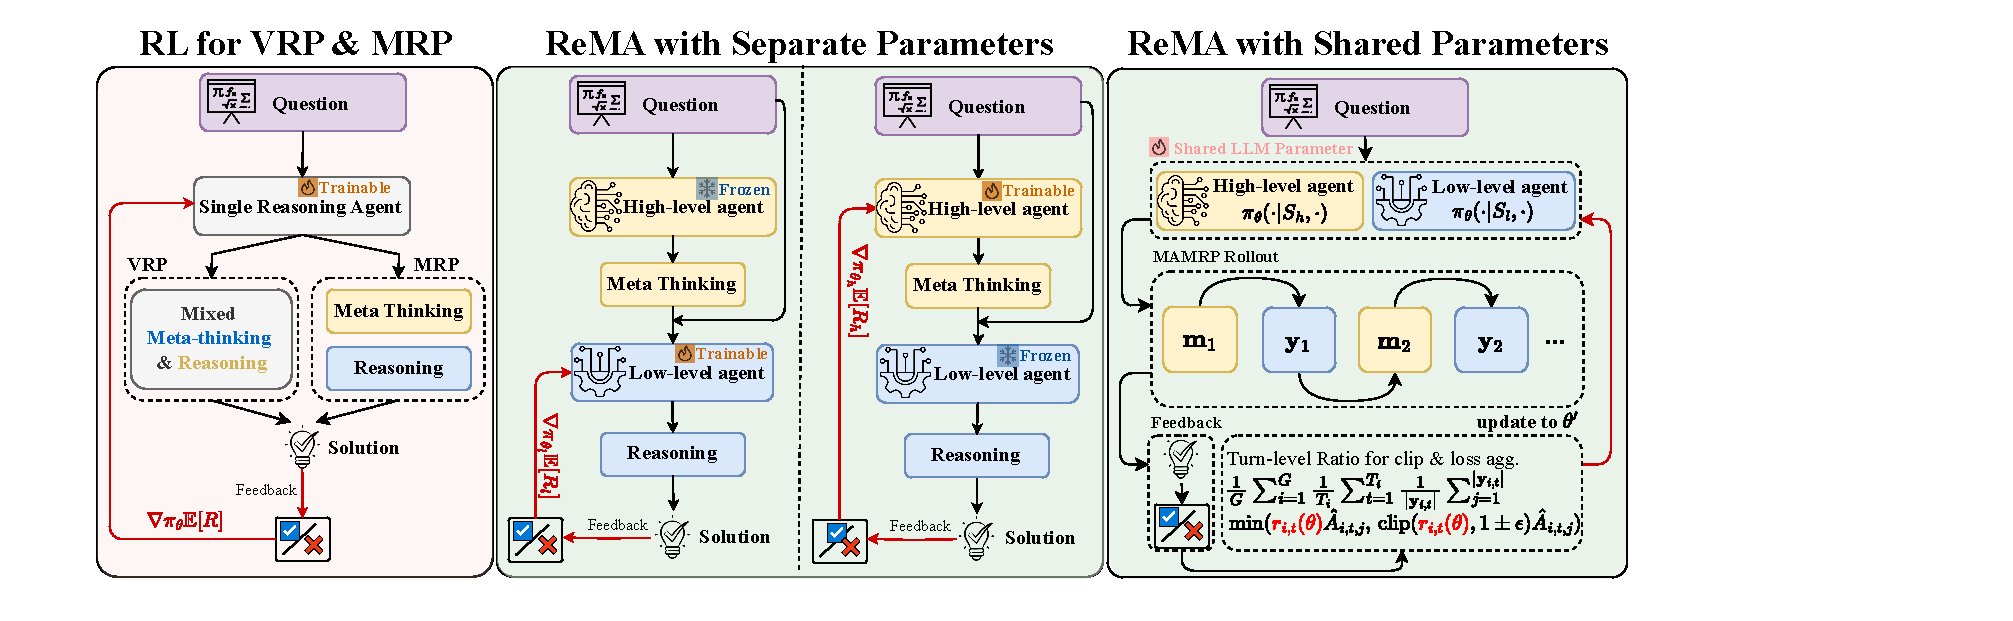
\includegraphics[width=1.0\linewidth]{figures/mainv3/train4.pdf}
    \vspace{-10pt}
    \caption{
Comparison of training pipelines. 
\textbf{Left:} RL training of VRP and MRP, where a single LM agent is updated either with mixed (VRP) or explicit (MRP) meta-thinking. 
\textbf{Middle:} \method{} with separate parameters for the high-level (meta-thinking) and low-level (reasoning) agents; training alternates between freezing one agent and updating the other. 
\textbf{Right:} \method{} with shared parameters and multi-turn interactions: both agents share the same parameters and are distinguished by their system prompts. Training employs a turn-level ratio for stable multi-turn reinforcement learning and efficient updates, ensuring each turn’s contribution is controlled to prevent instability.
}
    \label{fig:rl_train}
    \vspace{-10pt}
\end{figure}

\subsubsection{Scaling up to Multi-turn MAMRP}
\label{sec:method.reinforce_ma.multi_turn}

% Given the objective function, we apply the RL methods introduced in Section \ref{sec:preliminaries.rl} to optimize both agents. In practice, we compute each model's policy gradients and update their parameters jointly. When computational budget or training time is constrained, we alternatively freeze one agent and train only the other. To stabilize the training process, we propose a multi-turn Group Relative Policy Optimization algorithm with turn-level clipping to address these challenges.

To scale up to multi-turn MAMRP, we can still adopt the iterative training strategy in Sec.~\ref{sec:method.reinforce_ma.single_turn}. However, we make some changes to improve the efficiency of rollout and training.

First, we implement a parameter-sharing strategy where both high-level and low-level agents utilize identical model weights $\theta$, distinguished only by role-specific system prompts $S_h$ and $S_l$. Formally, we define $\pi_h = \pi_\theta(\cdot|S_h, \cdot)$ and $\pi_l = \pi_\theta(\cdot|S_l, \cdot)$, sharing the same underlying parameters rather than maintaining separate model instances. 
% We maintain two message lists for each agent in which they act as the assistant and follow the role-specific system prompts.
This approach eliminates the need for frequent model swapping on GPU during rollout, avoiding inefficient wait times, while enabling larger batch sizes during training to simultaneously optimize policies for both meta-thinking and reasoning roles. 
% It also leverages the inherent versatility of larger-scale models, which demonstrate superior capability in handling diverse tasks across different reasoning roles.

Second, we propose a multi-turn GRPO with \textbf{turn-level ratio} to address the challenges of multi-turn MAMRP.
The trajectory-level averaged objective with \textbf{turn-level ratio} of $\pi_l$ is defined as (The objective of $\pi_h$ is the similar but with different system prompt):
{\small
\begin{equation}
\begin{aligned}
\mathcal{J}(\theta) &= \mathbb{E}_{(\mathbf{x},\mathbf{y}^*)\sim\mathcal{D},\, \{(\mathbf{m}_i, \mathbf{y}_i)\}_{i=1}^G \sim \pi_{\theta_{\mathrm{old}}}(\cdot|\mathbf{x})} 
\\
&\Bigg[
\frac{1}{G} \sum_{i=1}^G \frac{1}{T_i} \sum_{t=1}^{T_i} \frac{1}{|\mathbf{y}_{i,t}|} \sum_{j=1}^{|\mathbf{y}_{i,t}|}
\Big(
\min({\color{red}r_{i,t}(\theta)} \hat{A}_{i,t,j},\, \mathrm{clip}({\color{red}r_{i,t}(\theta)}, 1-\epsilon, 1+\epsilon) \hat{A}_{i,t,j})
- \beta D_{\mathrm{KL}}(\pi_\theta \| \pi_{\mathrm{ref}})
\Big)
\Bigg]
\end{aligned}
\end{equation}
}
where $\mathbf{y}_{i,t,j}$ is the $j$-th token at turn $t$ of the reasoning agent of the $i$-th trajectory. And the turn-level ratio for clipping is defined as:
\begin{align}
    r_{i,t}(\theta)
    &= \frac{1}{|\mathbf{y}_{i,t}|}\sum\limits_{j=1}^{|\mathbf{y}_{i,t}|} r_{i,t,j}(\theta)
    =\frac{1}{|\mathbf{y}_{i,t}|}\sum\limits_{j=1}^{|\mathbf{y}_{i,t}|}
    \frac{
    \pi_\theta
    \bigl(
        \mathbf{y}_{i,t,j}\mid \mathbf{x}, \{\mathbf{m}_{i,\cdot}, \mathbf{y}_{i, \cdot}\}_{<t},  \mathbf{m}_{i, t}, \mathbf{y}_{i,t,<j}
    \bigr)
    }{
    \pi_{\theta_{\mathrm{old}}}
        \bigl(
            \mathbf{y}_{i,t,j}\mid \mathbf{x}, \{\mathbf{m}_{i,\cdot}, \mathbf{y}_{i, \cdot}\}_{<t},  \mathbf{m}_{i, t}, \mathbf{y}_{i,t,<j}
        \bigr)
    }.
    \label{eq:turn_grpo}
\end{align}
The introduction of the turn-level ratio serves two key purposes. 
First, using a token-level ratio (Eq.~(\ref{eq:grpo})) in the objective introduces bias for multi-turn training, as it averages over all tokens in a trajectory. This means that tokens within longer turns (those containing more tokens) can disproportionately influence the overall loss, and averaging at the token level may encourage excessively long single-turn responses. Second, clipping each token independently risks instability during training.

In contrast, the turn-level ratio aligns more closely with the underlying MDP formulation by treating all tokens within a turn as a single action and applying clipping at the turn level.
Intuitively, this approach stabilizes training by preventing the LLM from making unstable updates that could result in extreme outputs, such as overly long repetitions or incoherent text.
We conduct experimental verification in subsequent empirical results (Sec.~\ref{sec:exp.multiturn}).
% \ziyu{"Additionally, we clip extreme values after computing log ratios to maintain numerical stability." this line can be moved to appendix}
% This prevents the LLM from producing unstable updates caused by generating extreme outputs, such as excessively long repetitions or garbled text.

% \ziyu{This paragraph and the above objective is for multi-turn, I think we can first describe how we train single turn ReMA with separated parameters. And then to scale ReMA up, we adopt Parameter Sharing, GRPO and clipping.}

% To improve the training process, we consider model sizes and training efficiency, we propose a parameter-sharing approach where both high-level and low-level agents utilize the same model weights $\theta$ but with distinct role-specific system prompts $S_h$ and $S_l$, respectively. Formally, we denote $\pi_h = \pi_\theta(\cdot|S_h, \cdot)$ and $\pi_l = \pi_\theta(\cdot|S_l, \cdot)$ sharing the same underlying model parameters, rather than maintaining two separate full model instances. This approach not only reduces computational overhead but also leverages the inherent versatility of larger-scale models, which demonstrate superior capability in handling diverse tasks across different reasoning roles.

% Additionally, to stabilize the training process, we conduct prompt filtering as described in \citet{cui2025prime}: 
% during each round of training, we filter out the questions that our models solve with a success rate less than $\varepsilon_{\min}$ or greater than $\varepsilon_{\max}$.
% Similar to \citet{kirchner2024proververifiergamesimprovelegibility}, we train the models iteratively with RL algorithms as shown in the Algorithm \ref{alg:MAMRP_training}. \yx{TODO: add algorithm 2?}

% \subsection{Scaling up ReMA}
% \label{sec:method.reinforce_ma.extend_ma}

% To scale up ReMA, there are several key considerations: (1) enlarging model sizes to improve reasoning capabilities; (2) expanding dataset diversity and scale for better generalization; (3) addressing computational challenges during training and inference through efficient resource management techniques like distributed training and optimization; (4) Beyond the single-turn MAMRP detailed in Section \ref{sec:method.reinforce_ma.deploy_ma}, ReMA can be extended to multi-turn reasoning scenarios where agents collaborate to find the best solution.
% We will focus on the latter two aspects in this section.

% First, when considering model sizes and training efficiency, we propose a parameter-sharing approach where both high-level and low-level agents utilize the same model weights $\theta$ but with distinct role-specific system prompts $S_h$ and $S_l$, respectively. Formally, we denote $\pi_h = \pi_\theta(\cdot|S_h, \cdot)$ and $\pi_l = \pi_\theta(\cdot|S_l, \cdot)$ sharing the same underlying model parameters, rather than maintaining two separate full model instances. This approach not only reduces computational overhead but also leverages the inherent versatility of larger-scale models, which demonstrate superior capability in handling diverse tasks across different reasoning roles.

% Next, we extend MAMRP to multi-turn settings. In multi-turn MAMRP, the process follows an iterative pattern where the high-level agent $\pi_h$ and low-level agent $\pi_l$ exchange information multiple times to refine the solution. We formalize this as:
% \begin{equation}
%     \mathbf{y}_T 
%     \sim 
%     \pi_l(\mathbf{y}_T|\mathbf{x}, \ldots, \mathbf{m}_T) \cdot \pi_h(\mathbf{m}_T|\mathbf{x}, \ldots, \mathbf{y}_{T-1}, \mathbf{m}_{T-1}) 
%     \cdot \ldots \cdot 
%     \pi_l(\mathbf{y}_1|\mathbf{x}, \mathbf{m}_1) \cdot \pi_h(\mathbf{m}_1|\mathbf{x}),
%     \label{eq:multi_turn_mamrp}
% \end{equation}

% where $T$ is the number of turns, $\mathbf{m}_t$ represents the meta-thinking at turn $t$, and $\mathbf{y}_t$ represents the reasoning steps and intermediate solution at turn $t$. This can be visualized as:
% \begin{equation}
%     \mathbf{x} \xrightarrow[\pi_h]{\text{meta-thinking}} \mathbf{m}_1
%     \xrightarrow[\pi_l]{\text{reasoning}} \mathbf{y}_1 
%     \xrightarrow[\pi_h]{\text{meta-thinking}} \mathbf{m}_2
%     \xrightarrow[\pi_l]{\text{reasoning}} \mathbf{y}_2 
%     \xrightarrow[\pi_h]{\text{meta-thinking}} ... 
%     \xrightarrow[\pi_l]{\text{reasoning}} \mathbf{y}_T 
%     \sim
%     \mathbf{a}.
%     \label{eq:multi_turn_mamrp_graph}
% \end{equation}

% Compared to VRP and MRP which are deterministic MDPs, such a multi-turn pattern introduces more stochasticity. Moreover, non-stationarity to the training process makes it even harder to train. 
% We propose a multi-turn Group Relative Policy Optimization algorithm with turn-level clipping to address these challenges.
% The main idea is originated from GRPO \citep{shao2024deepseekmath} and is adapted for multi-turn MAMRP. 
% Our ultimate goal is to optimize the expected outcome of a trajectory $\tau = (\mathbf{x}, \mathbf{y}_1, \mathbf{m}_1, \mathbf{y}_2, \mathbf{m}_2, ..., \mathbf{y}_T, \mathbf{m}_T \sim \mathbf{a})$ on the training dataset $\mathcal{D}$.
% We denote the $j$-th token at turn $t$ of the reasoning agent of the $i$-th trajectory as $\mathbf{y}_{i,t,j}$. And $\mathbf{m}_{i,t,j}$ of a similar meaning.
% Then we denote the \textbf{trajectory-level averaged} and \textbf{turn-level clipped} training objective of $\pi_l$ as:
% \begin{align}
%     L(\theta)
%     =
%     &\mathbb{E}_{(\mathbf{x,y^*})\sim\mathcal{D},\;\{(\mathbf{m}_i, \mathbf{y}_i)\}_{i=1}^G\sim\pi_{\theta_{\mathrm{old}}}(\cdot\mid \mathbf{x})}\nonumber\\
%     &\Biggl[
%         \frac{1}{G}
%         \sum_{i=1}^G
%         \frac{1}{T_i}
%         \sum_{t=1}^{T_i}
%         \frac{1}{\lvert \mathbf{y}_{i,t}\rvert}
%         \sum_{j=1}^{\lvert \mathbf{y}_{i,t}\rvert}
%         \Bigl(
%             \min\bigl({\color{red}r_{i,t}(\theta)}\,\hat A_{i,t,j},\,
%             \mathrm{clip}\bigl({\color{red}r_{i,t}(\theta)},\,1-\epsilon,\,1+\epsilon\bigr)\,\hat A_{i,t,j}\bigr) \nonumber\\
%             &-\beta\,D_{\mathrm{KL}}\bigl(\pi_\theta\|\pi_{\mathrm{ref}}\bigr)
%         \Bigr)
%     \Biggr],
%     \label{eq:multi_turn_loss}
% \end{align}
% where the turn-level ratio for clipping is defined as:
% \begin{align}
%     r_{i,t}(\theta)
%     &= \frac{1}{|\mathbf{y}_{i,t}|}\sum\limits_{j=1}^{|\mathbf{y}_{i,t}|} r_{i,t,j}(\theta)
%     =\frac{1}{|\mathbf{y}_{i,t}|}\sum\limits_{j=1}^{|\mathbf{y}_{i,t}|}
%     \frac{
%     \pi_\theta
%     \bigl(
%         \mathbf{y}_{i,t,j}\mid \mathbf{x}, \mathbf{m}_{i,1}, \mathbf{y}_{i, 1}, \ldots, \mathbf{m}_{i, t}, \mathbf{y}_{i,t,<j}
%     \bigr)
%     }{
%     \pi_{\theta_{\mathrm{old}}}
%         \bigl(
%             \mathbf{y}_{i,t,j}\mid \mathbf{x}, \mathbf{m}_{i,1}, \mathbf{y}_{i, 1}, \ldots, \mathbf{m}_{i, t}, \mathbf{y}_{i,t,<j}
%         \bigr)
%     }.
% \end{align}
% Instead of clipping at the token-level to maximize the sample efficiency, we conservatively clip at the turn-level to ensure the stability of the training process. 
% This prevents the LLM from producing unstable updates caused by generating extreme outputs, such as excessively long repetitions or garbled text.

